\documentclass[a4paper,10pt,oneside]{report}%pridat twoside, do [] pre obojstrannu tlac
\pagestyle{headings}
\usepackage[top=2.5cm, bottom=2.5cm, left=3.5cm, right=2cm]{geometry} %odporucane okraje
\linespread{1.50}

%% Generally used
\usepackage{ebproof}
\usepackage{amsthm}
\usepackage{amsmath}
\usepackage{amssymb, upgreek}
\usepackage{mathtools}
\usepackage{color}
%% Generally used

%% Lean specific
\usepackage[utf8x]{inputenc}
\definecolor{keywordcolor}{rgb}{0.7, 0.1, 0.1}   % red
\definecolor{commentcolor}{rgb}{0.4, 0.4, 0.4}   % grey
\definecolor{symbolcolor}{rgb}{0.0, 0.1, 0.6}    % blue
\definecolor{sortcolor}{rgb}{0.1, 0.5, 0.1}      % green
\definecolor{errorcolor}{rgb}{1, 0, 0}           % bright red
\definecolor{stringcolor}{rgb}{0.5, 0.3, 0.2}    % brown
\usepackage{pict2e,picture}

\usepackage{listings}
\def\lstlanguagefiles{lstlean.tex}
\lstset{language=lean}
%% Lean specific

%% Covering

\newcommand{\coveringA}{%
  \mathrel{-\mkern-4mu}<%
}
\newcommand{\coveringB}{\mathrel{\text{$\vcenter{\hbox{\pictcoveringB}}$}}}

\newcommand{\pictcoveringB}{%
  \begin{picture}(1em,.5em)
  \roundcap
  \put(0,.25em){\line(1,0){.6em}}
  \put(.6em,.25em){\line(3,1){.4em}}
  \put(.6em,.25em){\line(3,-1){.4em}}
  \end{picture}%
}
%% Covering

%% Powerset
\newcommand{\powerset}{\raisebox{.15\baselineskip}{\Large\ensuremath{\wp}}}
%% Powerset
\newcommand{\nothing}{\varnothing}

\newtheorem{theorem}{Theorem}


\author{Mat\'u\v{s} Behun}
\title{Lattice theory notes}

\begin{document}

\tableofcontents

\section{Úvod}

%Pri procese rozširovania matematickej teórie vytvárame tvrdenia generalizujúce jej princípy.
%Ak chceme aby náša teória bola správna, všetky jej tvrdenia musia byť logicky odvodené z postulátov alebo tvrdení z nich odvodených.
%Potvrdenie správnosti tvrdenia, vyslovením predpokladu, axiómu alebo napísaním formule ktorú dostaneme aplikáciou dedukčného pravidla na niektoré v postupnosti predchádzajúce formule nazývame dôkazom.

%% Je to pravda?
%Z kvalitatívneho hľadiska pri vyslovení dôkazu uvažujeme o všeobecnosti dôkazu a správnosti aplikácie dedukčného pravidla.
%% Je to vhodný príklad(chcel som uviest priklad na prvy pohlad spravneho tvrdenia ktore bolo dokazane ako nespravne ? Ako správne citovať? Nápad som mal odtiaľto https://en.wikipedia.org/wiki/List_of_disproved_mathematical_ideas
%O nutnosti korektného dokazovania tvrdení hovorí napríklad tvrdenie z teórie čísel o hornom ohraničení počtu prvočísel logaritmickým integrálom.

%\begin{equation}
    %\pi(x) \leq \int_{0}^{x} \frac{1}{ \ln{t} } dt
%\end{equation}

%Tvrdenie bolo považované za správne Bernhardom Riemannom a evidencia to taktiež naznačovala.
%Neskôr sa ukázalo že tvrdenie nie je správne pri čísle pod hodnotou $10^{317}$.
%% Doplniť rok
%Veta o 4 farbách ktorá bola vyslovená v roku 1852 Francisom Guthrie ktorá hovorí, že každá rovinná mapa je zafarbiteľná 4 farbami.
%% 18-faces
%Táto veta bola nesprávne dokázaná v roku Kempom (1879) and Taitom (1880). Kempov dôkaz bol vyvrátený o 10 rokov mapov s 18 stenami.
%% Je lepšie skloňovať cudzie mená?
%Pri dôkaze tejto vety bol neskôr v roku 1977 Appelom and Hakenom z časti využitý počítač pre kontrolu špeciálnych diskrétnych prípadov.


\section{Prirodzená intuionistická logika}

\subsection{Formalizovanie dôkazu}

Dôkaz z teórie usporiadania. Tak ako je Program = Proof

Otázka ohľadom konzistentnosti dôkazu.

\subsection{Prirodzená dedukcia}

% Formula vyrokoveho poctu
\begin{theorem}[Výroková premenná, formula]
    Majme spočítateľnú množinu $\mathcal{X}$ výrokových premenných. Množina výrokov
    alebo formúl $\mathcal{A}$ generovanú nasledovnou gramatikou:
    \begin{equation}
        A, B ::= X | A \implies B | A \wedge B | A \vee B | \neg A | \top | \bot
    \end{equation}
    Kde $X \in \mathcal{X}$ reprezentuje výrokovú premennú, a $A, B \in \mathcal{A}$
    výrok.
\end{theorem}

V prípade nasledovného výroku je precedencia $\neg$ vyššia ako $\vee$ alebo $\wedge$
a tá je vyššia ako $\implies$. Binárne operátory sú asociatívne z prava.

\begin{align*}
    \neg A \wedge B \wedge C &\implies A \vee B \\
    (\neg A \wedge (B \wedge C)) &\implies (A \vee B) \\
\end{align*}

\begin{theorem}
    Kontextom(systém predpokladov) rozuemieme zoznam výrokov značených
    \begin{equation}
        \Gamma = P_{1}, \dots , P_{n}
    \end{equation}
    Dedukciou nazývame dvojicu pozostávajúcu z kontextu a výroku.
    \begin{equation}
        \Gamma \vdash A
    \end{equation}
\end{theorem}

Výraz čítame ako $A$ je možné dokázať zo systému predpokladov $\Gamma$.

\begin{theorem}
    Dedukčné pravidlo pozostáva z množiny dedukcií $\Gamma_{i}$ ktoré nazývame
    prepokladom. Dolnú časť dedukčného pravidla $\Gamma$ nazývame záverom.
    \begin{equation}
        \begin{prooftree}
            \hypo{\Gamma_{1} \vdash A_{1}}
            \hypo{\dots}
            \hypo{\Gamma_{n} \vdash A_{n}}
            \infer3[]{\Gamma \vdash A}
        \end{prooftree}
    \end{equation}
\end{theorem}
Pravidlá prirodzenej intuicionistickej logiky:
\begin{center}
    \begin{prooftree}
        \infer0[(ax)]{\Gamma,A,\Gamma' \vdash: A}
    \end{prooftree}
\end{center}
\vskip 0.2in
\begin{minipage}[t]{0.48\textwidth}
    \begin{prooftree}
        \hypo{\Gamma \vdash A \implies B}
        \hypo{\Gamma \vdash A}
        \infer2[$(\implies_{E})$]{\Gamma : B}
    \end{prooftree}
\end{minipage}
\hfill
\begin{minipage}[t]{0.48\textwidth}
    \begin{prooftree}
        \hypo{\Gamma, A \vdash B}
        \infer1[$\implies_{I}$]{\Gamma : B}
    \end{prooftree}
\end{minipage}
\vskip 0.2in
\begin{minipage}[t]{0.48\textwidth}
    \begin{prooftree}
        \hypo{\Gamma, A \vdash B}
        \infer1[$(\wedge^{l}_{E})$]{\Gamma : A}
    \end{prooftree}
    \begin{prooftree}
        \hypo{\Gamma, A \vdash B}
        \infer1[$(\wedge^{r}_{E})$]{\Gamma : B}
    \end{prooftree}
\end{minipage}
\hfill
\begin{minipage}[t]{0.48\textwidth}
    \begin{prooftree}
        \hypo{\Gamma \vdash A}
        \hypo{\Gamma \vdash B}
        \infer2[$(\wedge_{I})$]{\Gamma \vdash A \wedge B}
    \end{prooftree}
\end{minipage}
\vskip 0.2in
\begin{minipage}[t]{0.48\textwidth}
    \begin{prooftree}
        \hypo{\Gamma \vdash A \vee B}
        \hypo{\Gamma, A \vdash C}
        \hypo{\Gamma, B \vdash C}
        \infer3[$(\vee_{E})$]{\Gamma \vdash C}
    \end{prooftree}
\end{minipage}
\hfill
\begin{minipage}[t]{0.48\textwidth}
    \begin{prooftree}
        \hypo{\Gamma \vdash B}
        \infer1[$(\vee_{I}^{r})$]{\Gamma \vdash A \vee B}
    \end{prooftree}
    \begin{prooftree}
        \hypo{\Gamma \vdash A}
        \infer1[$(\vee_{I}^{l})$]{\Gamma \vdash A \vee B}
    \end{prooftree}
\end{minipage}
\vskip 0.2in
\begin{minipage}[t]{0.48\textwidth}
    \begin{prooftree}
        \hypo{\Gamma \vdash \neg A}
        \hypo{\Gamma \vdash A}
        \infer2[$(\neg_{E})$]{\Gamma \vdash \bot}
    \end{prooftree}
\end{minipage}
\hfill
\begin{minipage}[t]{0.48\textwidth}
    \begin{prooftree}
        \hypo{\Gamma, A \vdash \bot}
        \hypo{\Gamma \vdash A}
        \infer2[$(\neg_{I})$]{\Gamma \vdash \neg A}
    \end{prooftree}
\end{minipage}
\vskip 0.2in
\begin{center}
    \begin{prooftree}
        \hypo{\Gamma \vdash \bot}
        \infer1[$(\bot_{E})$]{\Gamma \vdash A}
    \end{prooftree}
\end{center}

V prípade že tieto pravidlá čítame zhora nadol hovoríme o dedukcii.
Ak čítame pravidlá zdola nahor hovoríme o indukčnom spôsobe.

\begin{theorem}
    Fragmentom intuionistickej logiky nazývame, systém ktorý dostaneme ak ho obmedzíme
        len na niektoré z predchádzajúcich pravidiel.
\end{theorem}

\begin{theorem}
    Implikačným fragmentom intuionistickej logiky dostaneme v prípade ak formuly
        budú tvorené gramatikou
    \begin{equation}
        A,B ::= X | A \implies B
    \end{equation}
    a pravidlami (ax), ($\implies_{E}$), ($\implies_{I}$)
\end{theorem}

% TODO spravit priklad
% (𝐴∧𝐵)→((𝐴→𝐶)→¬(𝐵→¬𝐶))

V prípade že chceme aby výrokove formuly korenšpondovali s typmi ktoré su prezentované neskôr.
Ich booleova reprezentácia s hodnotami $1,0$ je nahradená otázkou existencie prvkov v množine.
V prípade implikácie o existencii funkcie v množine.
Funkcie v programoch ale môžu mať pri rovnakých vstupoch a výstupoch mať rôznu výpočtovú zložitosť.
Dôvod prečo by sme sa mali pozerať na dôkazy(podľa publikácie Gir11) v troch rovinách.

\begin{itemize}
    \item 1. Booleovský - tvrdenia sú booleovské hodnoty, zaujímame sa o dokázateľnosť tvrdenia
    \item 2. Existenčný - tvrdenia sú množiny, aké funkcie môžu byť
    \item 3. Úmyselný/Zámerový(Intentional) - zaujímame sa o zložitosť vytvoreného dôkazu a ako sa zjednoduší cez (cut eliminitation)
\end{itemize}

\subsection{Intuicionizmus}

Jedným zo smerov matematickej filozofie týkajucej sa rozvoja teórie je konštruktivizmus.
Konštruktivizmus hovorí o potrebe nájsť alebo zostrojiť matematický objekt k tomu
    aby bola dokázaná jeho existencia.
Jeden z motivačných príkladov takéhoto prístupu je možnosť dokázania pravdivosti
výroku $p \vee \neg p$ cez dôkaz sporom $\neg p$ ktorý nehovorí ako zostrojiť objekt
$p$ len o jeho existencii.
Tento smer tvorí viacero "škôl" okrem iných finitizmus, predikativizmus, intuicionizmus.
Intuitionizmus je teda konštruktívny prístup k matematike v duchu
    Brouwera(1881-1966) a Heytinga(1898-1980).
Filozofickým základom tochto prístupu princíp že matematika je výtvorom mentálnej
činnosti a nepozostáva z výsledkov  formálnej manipulácie symbolov ktoré sú iba
sekundárne.
Jedným z princípov intuicionizmus je odmietnutie tvrdenia postulátu klasickej
logiky a to zákona vylúčenia tretieho.

\begin{equation}
    p \vee \neg p
\end{equation}

Dôvodom je z konštruktívneho pohľadu nezmyselnosť uvažovania nad pravdivosťou
    výroku nezávisle od uvažovaného tvrdenia.
Výrok je teda pravdivý ak existuje dôkaz o jeho pravidovsti a nepravdivé
    ak existuje dôkaz ktorý vedie k sporu.

\begin{itemize}
    \item konjukcii $ p \wedge q $ ako o výroku hovoriacom o existencii dôkazov $p$ a zároveň $q$,
    \item disjunkcii $ p \wedge q $ ako existencii konštrukcii dôkazu jedného z výrokov $p, q$,
    \item $ p \implies q $ je metóda(funkcia) transformácie každej konštrukcie $p$ k dôkazu $q$,
    \item neexistencie dôkazu nepravdivého tvrdenia, iba dôkazu ktorý vedie k sporu $p \implies \bot$
    \item konštrukcia $\neg p$ je metóda ktorá vytvorí každú konštrukciu $p$ na neexistujúci objekt
\end{itemize}

konjukcii $ A \wedge B $ ako $ A \times B $
$ A \vee B $ ako $ A \sqcup B $ disjunktne zjednotenie
$ \neg A = A \implies \perp $ existencie kontrapríkladu

\section{Lambda kalkulus}

\begin{theorem}
    Majme nekonečnú množinu $ \mathcal{X}={x,y,z,\dots}$ ktorých elementy nazývame premenné.
Množinu $\Lambda$ tvorenú $\lambda$-termínmy je potom generovaná nasledovnou gramatikou:
    \begin{equation}
        t, u ::= x | t u | \lambda x.t
    \end{equation}
\end{theorem}
\noindent Význam jednotlivých termínov je
\begin{align*}
     x          & \textrm{ - je premennou }\\
     t u        & \textrm{ - je aplikáciou termínu $t$ s argumentom $u$ }\\
    \lambda x.t & \textrm{ - je abstrakciou $t$ nad $x$ }
\end{align*}
Príklady lambda termínov:

\begin{align*}
    & t x \\
    & (\lambda y . \lambda x . t y )) \\
    & (\lambda y.y x) (\lambda x . x) \\
    & t u v = ( t u ) v
\end{align*}

Aplikácia $\lambda$-termínov je implicitne aplikovaná zľava.

Pri výraze
\begin{equation}
    \lambda x . t x = \lambda x . (t x)
\end{equation}
je precedencia aplikácie vyššia ako abstrakcia.

A abstrakciu s troma argumentmi je možné prepísať do troch po sebe nasledujúcich.
\begin{equation}
    \lambda x y z . t = \lambda x . \lambda y . \lambda z . t
\end{equation}

\begin{theorem}
    Premenná x sa vo výraze
    \begin{equation}
        \lambda x . t
    \end{equation}
    abstrakciou viaže na termín $t$. O premennej $x$ hovoríme že je viazaná.
    O premenných ktoré nie sú viazané sú voľné.
    \begin{align*}
        VP(x) &= {x} \\
        VP(\lambda x.t) &= VP(t)  \setminus \{x\} \\
        VP(t v) &= VP(t) \cup VP(v)
    \end{align*}
\end{theorem}

\begin{theorem}
    Premenovaním nazývame nahradenie voľných premenných v termíne.
    \begin{equation}
        t \{ y / x \}
    \end{equation}
\end{theorem}
V termíne $t$ je premenovaná premenná $x$ za $y$.

% TODO pridaj priklady
\subsection{$\alpha$-ekvivalencia}
\begin{theorem}
    O výrazov hovoríme že sú alfa-ekvivalentné ak sa výrazy rovnajú až na premenovanie.
\end{theorem}

\begin{theorem}
    O substutícii hovoríme pri nahradení jednej premenej druhou.
    \begin{equation}
        t [ y / x ]
    \end{equation}
\end{theorem}

Nahradenie je silnejšie a vieme nahradiť aj premmenné viazanné abstrakciou.

\subsection{$\beta$-ekvivalencia}

\begin{minipage}[t]{0.48\textwidth}
    \begin{prooftree}
        \infer0[($\beta_{s}$)]{(\lambda x.t)u \to_{\beta} t [ u / x ]}
    \end{prooftree}
\end{minipage}
\hfill
\begin{minipage}[t]{0.48\textwidth}
    \begin{prooftree}
        \hypo{t \to_{\beta} t'}
        \infer1[($\beta_{\lambda}$)]{(\lambda x.t)u \rightarrow_{\beta} t [ u / x ]}
    \end{prooftree}
\end{minipage}
\vskip 0.2in
\begin{minipage}[t]{0.48\textwidth}
    \begin{prooftree}
        \hypo{t \to_{\beta} t'}
        \infer1[($\beta_{l}$)]{t u \rightarrow_{\beta} t' u}
    \end{prooftree}
\end{minipage}
\hfill
\begin{minipage}[t]{0.48\textwidth}
    \begin{prooftree}
        \hypo{u \to_{\beta} u'}
        \infer1[($\beta_{r}$)]{t u \rightarrow_{\beta} t u'}
    \end{prooftree}
\end{minipage}
\vskip 0.2in

% TODO vymysliet iny strom, tento je prevzaty
\begin{equation}
    \begin{prooftree}
        \infer0[($\beta_{s}$)]{(\lambda y.y)x \to_{\beta} x}
        \infer1[($\beta_{l}$)]{(\lambda y.y)xz \to_{\beta} xz}
        \infer1[($\beta_{\alpha}$)]{\lambda x.(\lambda y.y)xz \to_{\beta} \lambda x . xz}
    \end{prooftree}
\end{equation}

\begin{theorem}
    Definujme rekurziu volania funkcie nasledovne
    \begin{align}
        f^{0}x &= x \\
        f^{n}x &= f(f^{n-1}x) \\
    \end{align}
    Potom Churchove číslo $c_{n}$ je $\lambda$-termín
    \begin{equation}
        c_{n} = \lambda s . \lambda z . s^{n} (z)
    \end{equation}
\end{theorem}

Prirodzené čísla je potom definovať
\begin{align*}
    0 &= \lambda f x . x \\
    1 &= \lambda f x . f x \\
    1 &= \lambda f x . f (f x) \\
    2 &= \lambda f x . f ( f (f x))
\end{align*}

\begin{align*}
    succ(n) &=           (\lambda n f x .  f( n f x ))(\lambda f x . f^{n} x) \\
           &\to_{\beta} \lambda f x . f (( \lambda f x . f^{n} x ) f x)      \\
           &\to_{\beta} \lambda f x . f (( \lambda x . f^{n} x) x)           \\
           &\to_{\beta} \lambda f x . f (f^{n} x)                            \\
           &=           \lambda f x . f^{n+1} x                              \\
           &= n + 1
\end{align*}

Operáciu sčítania je potom možné definovať vykonať
\begin{theorem}
    $f_{+} = \lambda x. \lambda y. \lambda s. \lambda z. x s (y s z)$
\end{theorem}

Podobným spôsobom môžeme vytvoriť 
\begin{theorem}
    \begin{align*}
        True &= \lambda x y . x \\
        False &= \lambda x y . y
    \end{align*}
\end{theorem}

\begin{align*}
    if = \lambda b x y . b x y
\end{align*}

\begin{align*}
    if \textrm{ True } t u = (\lambda bxy.bxy)(\lambda xy.x) tu & \to_{\beta} (\lambda xy.(\lambda xy.x)xy)tu \\
                                                     & \to_{\beta} (\lambda y.( \lambda xy.x)ty)u \\
                                                     & \to_{\beta} (\lambda xy.x)tu \\
                                                     & \to_{\beta} (\lambda y.t)u \\
                                                     & \to_{\beta} t
\end{align*}

\begin{theorem}
    Jednoduchý $\lambda$ kalkulus je ekvivalentný výpočtovej sile turingovho stroja.
    Bez dôkazu
\end{theorem}

\section{Typovo jednoduchý $\lambda$-calculus}

Typový lambda calculus je rozšírením jednoduchého o typy

\begin{theorem}
    Majme množinu $U$ spočítateľnú nekonečnú abecedu obsahujúcu typové premenné.
    Potom množina $\Pi$ obsahuje reťazce jednoduchých typov ktoré su generované
    gramatikov:
    \begin{equation}
        \Pi ::= U | (\Pi \to \Pi)
    \end{equation}
\end{theorem}

\begin{theorem}
    Kontextom rozumieme množinu $C$ tvoriacu 
    \begin{equation}
        { x_{1} : \tau_{1}, \dots, x_{n} : \tau_{n} }
    \end{equation}
    kde $\tau_{1}, \dots, \tau_{n} \in \Pi$ a $x_{1}, \dots , x_{n} \in$
    Koobor kontextu je množina obsahujúca
    \begin{equation}
        domain(\Gamma) = { x_{1}, \dots, x_{n} }
    \end{equation}
    Oboor kontextu je množina obsahujúca
    \begin{equation}
        range( \Gamma ) = { \tau \in \Pi  | (x : \tau ) \in \Gamma }
    \end{equation}
\end{theorem}

\noindent Príklady generované gramatikou
\begin{itemize}
    \item $\vdash \lambda x.x : \sigma \to \sigma$
    \item $\vdash \lambda x. \lambda y.x : \sigma \to \tau \to \sigma$
    \item $\vdash \lambda x. \lambda y. \lambda z.x z (y z): (\sigma \to \tau \to \rho) \to (\rho \to \tau) \to \sigma \to \rho$
\end{itemize}

\begin{theorem}
    Postupnosť je trojica značená
    \begin{equation}
        \Gamma \vdash t : A
    \end{equation}
tvorená kontextom $\Gamma$, $\lambda$-termínom $t$ a typom $A$.
\end{theorem}

Termín $t$ je typu $A$ ak v kontexte $\Gamma$ ak je postupnosť derivovateľná pomocou pravidiel:
\begin{itemize}
    \item ax: v kontexte $x$ je typu $A$
    \item $\overset{I}{\rightarrow}$: ak je $x$ typu $A$, $t$ je typu B, potom
        funkcia $\lambda x.t$ ktorá asociuje $x$ $t$ je typu $A \to B$
    \item $\overset{E}{\rightarrow}$: daná je funkcia $t$ je typu $A \to B$
        a argument $u$ je typu $A$, vysledok aplikácia $t u$ je typu $B$
\end{itemize}

\begin{center}
    \begin{prooftree}
        \infer0[ax]{\Gamma \vdash x : \Gamma(x)}
    \end{prooftree}
\end{center}
\vskip 0.2in
\begin{minipage}[t]{0.48\textwidth}
    \begin{prooftree}
        \hypo{\Gamma , x : A \vdash t : B }
        \infer1[$\overset{I}{\rightarrow}$]{\Gamma \lambda x^{A}.t : A \to B}
    \end{prooftree}
\end{minipage}
\hfill
\begin{minipage}[t]{0.48\textwidth}
    \begin{prooftree}
        \hypo{\Gamma \vdash t : A \to B }
        \hypo{\Gamma \vdash u : A }
        \infer2[$\overset{E}{\rightarrow}$]{\Gamma \vdash t u : B}
    \end{prooftree}
\end{minipage}

\section{Curry-Howardov izomorfizmus}

\begin{center}
    \begin{tabular}{ c c }
        Intuinistická logika & Typovo jednoduchý $\lambda$ kalkulus \\
        \hline
        termín                  & dôkaz \\
        typová premenná         & propozičná premenná \\
    \end{tabular}
\end{center}

\begin{theorem}{Curry-Howard isomorphism}
    \begin{itemize}
        \item If $\Gamma \vdash M : \varphi \textrm{ potom } |\Gamma|  \vdash \varphi.$
        \item If $\Gamma \vdash \varphi \textrm{ potom existuje } M \in \Lambda_{\Pi}
            \textrm{ také že } \Delta \vdash M : \varphi, \textrm{ kde }
            \Delta = { ( x_{\varphi} : \varphi ) | \varphi \in \Gamma }$
    \end{itemize}
\end{theorem}

\section{Počítačom asistované dokazovanie}
    To com som vravel v prezentacii, historia, na zaciatku sa pouzivalo
\section{Lean-theorem-prover}
    Lean je dokazovací asistent ktorý bol vytvorený otvorený softvérový projekt
Leonardom de Mourom v Microsoft Reasearch v roku 2013. Jazyk sa neustále vyvýja
a momentálne sa nachádza vo štvrtej iterácii zatiaľ čo komunitný projekt matematickej
knižnice mathlib sa stále vyvýja v tretej verzii.
\subsection{Constracting proof}

\subsection{Forward proofs}
    \subsubsection{assume}
    \subsubsection{calc}
    \subsubsection{fix}
    \subsubsection{have}
    \subsubsection{let}
    \subsubsection{show}
\subsection{Backward proofs}
    \subsubsection{cc}
    \subsubsection{clear}
    \subsubsection{exact}
    \subsubsection{induction}
    \subsubsection{intro}
    \subsubsection{refl}
    \subsubsection{refl}
\subsubsection{Inductive types}

\section{Teória usporiadania}
    V tejto kapitole sa budeme snažiť ukázať možnosti Lean-u a využitie už existujúcich
definícii v mathlibe pre dokázanie viet týkajúcich sa teórie usporiadania.
    Pre tento účel je Lean ideálny z pohľadu našich možností definovania vlastností
usporiadania, ktoré následne možno aplikovať na abstraktnú množinu objektov.
    % Toto by bolo dobré rozpracovať ďalej, možno konkrétny príklad
    Výsledný typ je potom odvodený na základe závislostných typov.
    Usporiadanie je jednoducho intuitívne uchopiteľná vlastnosť bez matematických
preddispozícií.
    V každodennom živote porovnávame svoju výšku, čas, ktorý trval na vybehnutie do kopca
alebo aj číselne neohodnotené, subjektívne merateľné objekty ako ktorý album
od skupiny preferujem.
    Na otázky si potom vieme odpovedať "ja som vyšší", "zabehol si pomalšie" alebo
tieto albumy sú neporovnateľné.

Teória usporiadania sa snaží tieto vlastnoti formálne definovať a rozvíjať ďalej
otázkami ako, aké je horné celej množiny objektov. Existuje ohraničenie horné alebo
dolné pre ľubovoľnú podmnožinu objektov?
    Pre stručnosť sa v rámcii definícii obmedzíme len na definíciu usporiadania
ako relácie, čiže podmnožinu karteziánskeho súčinu dvoch množín.

\begin{theorem}
    Majme množinu $P$, potom usporiadanie alebo čiastočné usporiadanie na množine
    $P$ je binárna relácia $\leq$ taká že, pre všetky $x,y,z \in P$
    \begin{itemize}
        \item $x \leq x$ vlastnoť reflexivity
        \item $x \leq y$ a $y \leq x$ implikuje $x = y$ antisymetria
        \item $x \leq y$ a $y \leq z$ impikuje $x \leq z$ tranzitivita
    \end{itemize}
\end{theorem}

    Ideálnym nástrojom pre uvažovanie nad usporiadaním sú \emph{Hasseho} diagramy.
    Ako príklad uvádzame diagram "kocky".

\begin{figure}[!ht]
    \centering
    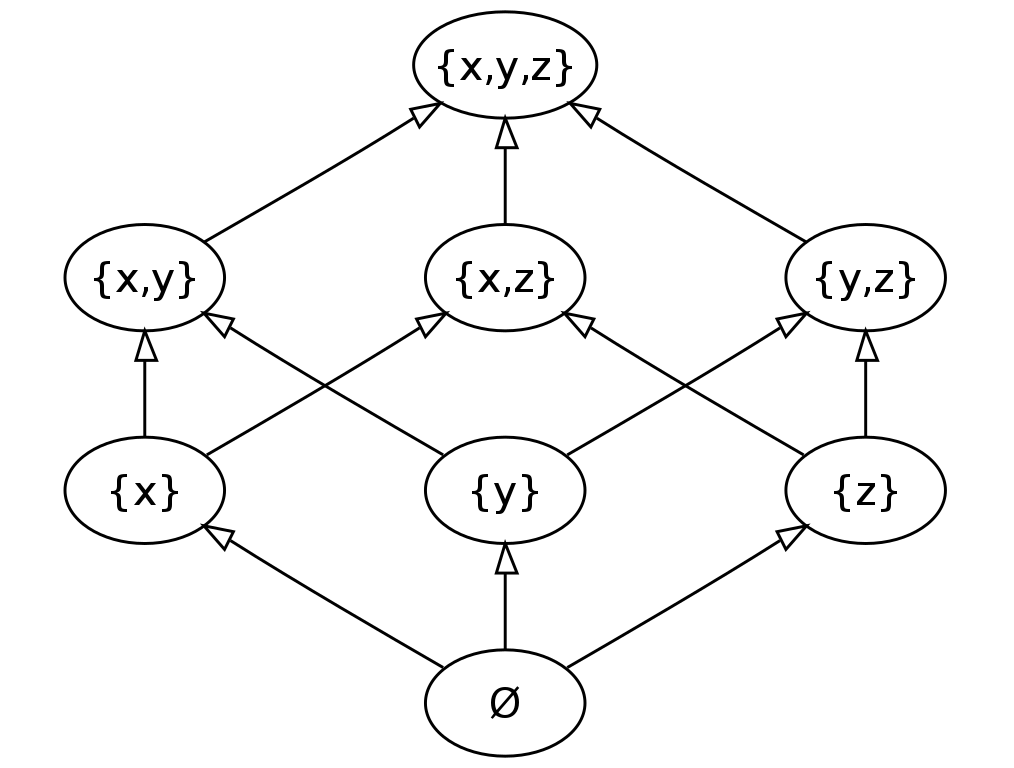
\includegraphics[scale=0.15]{cube.png}
    \caption{Usporiadania $\mathcal{P}(\{a,b,c\})$}
\end{figure}

    Na obrázku je usporiadanie množiny všetkých množín trojprvkovej množiny $\{ a,b,c \}$.
    Usporiadanie tvorí binárna relácia kardinality podmnožínm pričom porovnávame
len podmnožiny obsahujúce spoločný prvok.
    Vyššie sú položené väčšie prvky a porovnateľnými prvkami považujeme len tie,
ktoré sú "pokryté" jednosmernou cestou cez orientované hrany grafu.

    V Leane je usporiadanie definové ako rozšírenie triedy predusporiadania, ktorá
je reláciou, ktorá nemá oproti čiastočnému usporiadaniu vlastnosť antisymetrie.

\begin{lstlisting}
class has_le       (α : Type u) := (le : α → α → Prop)
class has_lt       (α : Type u) := (lt : α → α → Prop)

class preorder (α : Type u) extends has_le α, has_lt α :=
(le_refl : ∀ a : α, a ≤ a)
(le_trans : ∀ a b c : α, a ≤ b → b ≤ c → a ≤ c)
(lt := λ a b, a ≤ b ∧ ¬ b ≤ a)
(lt_iff_le_not_le : ∀ a b : α, a < b ↔ (a ≤ b ∧ ¬ b ≤ a) . order_laws_tac)
\end{lstlisting}
Čiastočné usporiadanie je potom rozšírením predusporiadania o vlastnosť antysymetrie.
\begin{lstlisting}
class partial_order (α : Type u) extends preorder α :=
(le_antisymm : ∀ a b : α, a ≤ b → b ≤ a → a = b)
\end{lstlisting}

DOPLN PRIKLAD NAJLEPSIE AK NAS USPORIADANY POSET Z PRIKLADU

\subsubsection{Zväz}
    Zväz je usporiadaná množina, pre ktorú navyše platí, že pre každé 2 prvky $a, b$
vieme nájsť prvok $c$, ktorý je ich jedinečným najmenším horným, respektíve(\emph{supremum})
najväčším dolným ohraničením(\emph{infinum}).
    V prípade intervalu reálnych čísel je toto ohraničenie jednoducho predstaviteľné
ako bod ohraničujúce množinu na číselnej osi.
    Ak ide o čiastočné usporiadanie, názov je pre tieto ohraničenia prvkov
motivovaný zobrezním na grafe.
    \emph{Spojenie} $\sqcup, \vee$ pre supremum, respektíve \emph{stretnutie} $\sqcap, \wedge$ pre infinum.
    Popisnejším názvom pre zväz je preklad anglicky používaného názvu \emph{lattice}
"mriežka" tak isto motivovaná zobrazením takého usporiadania na grafe.
    Pri dokazovaní viet o zväzoch je často využívaná vlastnosť duality najmenšieho
horného a duálne najväčšieho dolného ohraničenie pre druhú polovicu dôkazu.
    V prípade zväzu je táto vlastnosť využitá rovno v definícii zväzu ako spojenie
duálnej definície suprémoveho a infinumového semizväzvu.

\begin{lstlisting}
class has_sup (α : Type u) := (sup : α → α → α)
class has_inf (α : Type u) := (inf : α → α → α)

infix ⊔ := has_sup.sup
infix ⊓ := has_inf.inf

class semilattice_sup (α : Type u) extends has_sup α, partial_order α :=
(le_sup_left : ∀ a b : α, a ≤ a ⊔ b)
(le_sup_right : ∀ a b : α, b ≤ a ⊔ b)
(sup_le : ∀ a b c : α, a ≤ c → b ≤ c → a ⊔ b ≤ c)

class semilattice_inf (α : Type u) extends has_inf α, partial_order α :=
(inf_le_left : ∀ a b : α, a ⊓ b ≤ a)
(inf_le_right : ∀ a b : α, a ⊓ b ≤ b)
(le_inf : ∀ a b c : α, a ≤ b → a ≤ c → a ≤ b ⊓ c)

class lattice (α : Type u) extends semilattice_sup α, semilattice_inf α
\end{lstlisting}

Na nasledujúcich grafoch si ukážeme ako vyzerajú zväzy.

PRIDAT VLASTNY PRIKLAD, OPYTAT SA
\begin{lstlisting}
def poset_nat : sublattice ℕ :=
    { carrier := {n : ℕ | 1 ≤ n},
    inf_mem :=
      begin·
        intro a,
        intro b,
        intro a_set,
        intro b_set,
        simp at a_set,
        simp at b_set,
        simp,
        split,
        exact a_set,
        exact b_set,
      end,
    sup_mem := by finish,
}
\end{lstlisting}

\subsubsection{Modulárne zväzy}

V nasledujúcom úseku si ukážeme vetu týkajúcu sa špeciálneho typu zväzu s vlastnosťou
    modularity a ukážeme si formálny dôkaz a jej implementáciu v Leane, ktorú si
    podrobne rozoberieme.

O zväze $L$ hovoríme, že je modulárny, v prípade, že spĺňa nasledujúcu vlastnosť.

\begin{equation*}
    (\forall x,y,z \in L) x \geq y \implies x \wedge ( y \vee z) = (x \wedge y) \vee z
\end{equation*}

V Leane definovaný ako rozšírenie zväzu:

\begin{lstlisting}
class modular_lattice(α : Type u) extends lattice α :=
  (modular_law: ∀ (x u v : α ), (x ≤ u) → u ⊓ (v ⊔ x) = (u ⊓ v) ⊔ x )
\end{lstlisting}

V nasledujúcom úseku si ukážeme vetu o modulárnom izomorfizme a podrobne
    si rozoberieme implementáciu jej dôkazu s obsahom prostredia v Leane.

TODO ZJEDNOTIT ZNACENIE DEFINICIE A LEAN-u
\subsection{Modulárne zväzy}
    \begin{theorem} \emph{Veta o izomorfizme modulárnych zväzov}
    Nech L je modulárnym zväzom a $a, b \in L$. Potom
        \begin{equation}
            \varphi_{b}: x \mapsto x \wedge b, x \in [a, a \vee b],
        \end{equation}
    Je izomorfizmom medzi intervalmi $[a, a \vee b]$ a $[ a \wedge b, b]$.
    Inverzným izomorfizmom je
        \begin{equation}
            \psi_{a}: y \mapsto x \vee a, y \in [a \wedge b, b].
        \end{equation}
    \end{theorem}
    \emph{Dôkaz}.  Stačí ukázať, že $\varphi_{b}\psi_{a}(y) = y$ pre všetky $x \in [a, a \vee b]$.
    Z duality vyplýva, že $\varphi_{b}\psi_{a}(y) = y$ pre všetky
        $y \in [a \wedge b, b]$,
    Majme $x \in [a, a \vee b]$. Potom
        $\psi_{a}\varphi_{b} = ( x \wedge b ) \vee a$ nerovnosť $a \leq x$ platí
        potom aj modularita
        \begin{equation}
            \varphi_{a}\psi_{b}(x) =
            ( x \wedge b ) \vee a =
            x \wedge ( b \vee a) =
            x
        \end{equation}
        pretože
        \[
            \pushQED{\qed}
            x \leq a \vee b. \qedhere
            \popQED
        \]

    Predstavený dôkaz je znázornený na nasledujúcom grafe.

\begin{figure}[!ht]
    \centering
    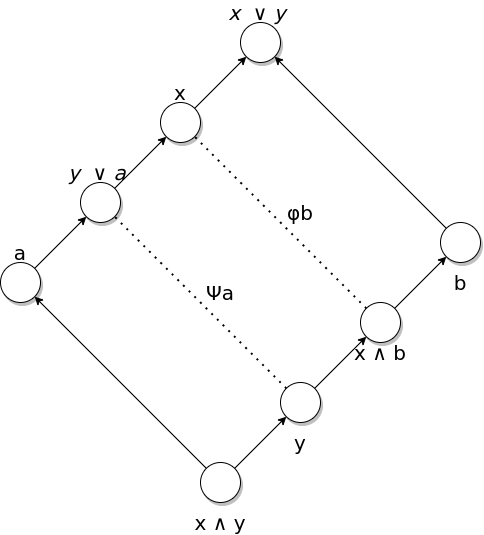
\includegraphics[scale=0.35]{modular_lattice_isomorphism.png}
    \caption{Izomorfizmus modulárneho zväzu}
\end{figure}

    V prípade formálneho dôkazu sme sa mohli v časti dôkazu odkázať na dualitu. 
    V prí návrhu dôkazu v Leane musím ukázať dôkaz z "oboch" strán.

\begin{lstlisting}
theorem modular_lattice_isomorphism { α: Type u } [ modular_lattice α ]
{ u v w x y : α } :
  x ≤ u →
  x ≥ v →
  x ≥ u ⊓ v →
  x ≤ u ⊔ v →
  u ⊓ ( v ⊔ x ) = x ∧ (u ⊓ x) ⊔ v = x
  :=
  begin
 1        intros h1 h2 h3 h4,
 2        split,
 3        {
 4          rw modular_lattice.modular_law,
 5          exact sup_eq_right.mpr h3,
 6          exact h1
 7        },
 8        {
 9          rw inf_comm,
10          rw ← modular_lattice.modular_law,
11          exact inf_eq_left.mpr h4,
11          exact h2
12        }
  end
\end{lstlisting}
    Začíname v taktickom móde prázdnou konštrukciou \emph{begin} a \emph{end}
    Interaktívne prostredie vyzerá nasledovne.
\begin{lstlisting}
α: Type u
_inst_1: modular_lattice α
u v w x y : α
⊢ x ≤ u → x ≥ v → x ≥ u ⊓ v → x ≤ u ⊔ v → u ⊓ (v ⊔ x) = x ∧ u ⊓ x ⊔ v = x
\end{lstlisting}
    Prvým krokom dôkazu je presunutie predpokladov zo sledu implikácii do
prostredia pre ďalšiu prácu s nimi s označením $h1,h2,h3,h4$.
\begin{lstlisting}
α: Type u
_inst_1: modular_lattice α
uvwxy: α
h1: x ≤ u
h2: x ≥ v
h3: x ≥ u ⊓ v
h4: x ≤ u ⊔ v
⊢ u ⊓ (v ⊔ x) = x ∧ u ⊓ x ⊔ v = x
\end{lstlisting}
    Cieľ potom pozostáva z konjukcie, kde v druhej časti máme výraz implicitne
ozátvorkovaný zľava.
    Výraz rozdelíme do dvoch podcieľov príkazom \emph{split}, a pre lepšiu
čitateľnosť ozátvorkujeme množinovými zátvorkami. Nachádzame sa v stave
\begin{lstlisting}
  begin
    intros h1 h2 h3 h4,
    split,
    {
    },
    {
    }
  end
\end{lstlisting}
v ktorom nám lean ukazuje prostredie, kde musíme dokázať ľavú časť konjukcie.
\begin{lstlisting}
⊢ u ⊓ (v ⊔ x) = x
\end{lstlisting}
Na cieľ použijeme z definície modulárneho zväzu vlastnosť modularity
\begin{lstlisting}
    (modular_law: ∀ (x u v : α ), (x ≤ u) → u ⊓ (v ⊔ x) = (u ⊓ v) ⊔ x )
\end{lstlisting}
a transformujeme prepíšeme cieľ cez príkaz
\begin{lstlisting}
rw modular_lattice.modular_law,
\end{lstlisting}
na nasledujúci, kde má $u \sqcap v$ vyššiu precedenciu
\begin{lstlisting}
⊢ u ⊓ v ⊔ x = x
\end{lstlisting}
    Nasledujúca transformácia vyžaduje znalosť už dokázaných definícií, ktoré
boli dokázané pre podkladové štruktúry. Použijeme nasledujúcu definíciu, ktorá vychádza
z kontextu \emph{semilattice\_sup}.
\begin{lstlisting}
% @[simp] theorem sup_eq_right : a ⊔ b = b ↔ a ≤ b :=    / TODO NEZABUDNUT
%  le_antisymm_iff.trans $ by simp [le_refl]             / ODKOMENTOVAT
    \end{lstlisting}
    Zaujímavosťou je, že si Lean dokáže substiuovať výraz $u \sqcap v$ za $a$ z uvedeného
výrazu. Pri použití vety dostávame ekvivalenciu, ktorá je definovaná ako štruktúra.
\begin{lstlisting}
structure iff (a b : Prop) : Prop :=
    intro :: (mp : a → b)
             (mpr : b → a)
\end{lstlisting}
Z tejto štruktúry použijeme implikáciu smerujúca doľava nasledovne:
\begin{lstlisting}
    exact sup_eq_right.mpr h3,
\end{lstlisting}
    Cieľ je teda transformovaný na:
\begin{lstlisting}
⊢ x ≤ u
\end{lstlisting}
čo je už uvedený predpoklad $h1$. Týmto sme dokázali jeden z podcieľov.
    V tejto chvíli by sme sa v literatúre mohli odvolať na dualitu výrazov.
    V Leane musíme poskytnúť dôkaz aj o druhom cieli. Ideme dokázať
\begin{lstlisting}
⊢ u ⊓ x ⊔ v = x
\end{lstlisting}
V tejto chvíli chceme znova použiť modularitu, leanu je, ale potrebné explicitne povedať,
    že chceme prepísať výraz nachádzajúci na pravej strane rovnosti pomocou symbolu
ľavej šípky.
\begin{lstlisting}
rw ← modular_lattice.modular_law,
\end{lstlisting}
    Použijeme duálnu vetu
    duálnu k \emph{sup\_eq\_right}.
\begin{lstlisting}
@[simp] theorem inf_eq_left : a ⊓ b = a ↔ a ≤ b
\end{lstlisting}
    a využijeme opačné predpoklady k predchádzajúcim $h2, h4$.
\begin{lstlisting}
{
    rw ← modular_lattice.modular_law,
    exact inf_eq_left.mpr h4,
    exact h2
}
\end{lstlisting}

Po dokázaní druhého cieľa sme dokázali celú vetu. $\square$

\begin{thebibliography}{xx}
    \bibitem{Mimram} Samuel Mimram, Program = Proof, Indenpendently published(July 3, 2020), ISBN-13: 979-8615591839
    \bibitem{SorensenUrzyczyn} Morten Heine B. Sørensen, Pawel Urzyczyn, Lectures on the Curry-Howard Isomorphism,
        Elsevier Science (April 4, 2013),  ISBN-13 : 978-0444545961
    \bibitem{}
\end{thebibliography}

Slovicka na ktore nepoznam preklad a ne
\begin{itemize}
    \item join - spojenie
    \item meet - stretnutie
\end{itemize}

\end{document}

\begin{verbatim}
    structure point :=
      ( x : nat )
      ( y : nat )

    /-- alternative notation -/
    structure point_alternative :=
      mk :: (x : nat) (Y : nat)

    def p1 : point :=
    {
      x   := 10,
      y   := 20,
    }

    /- same point, different notation, same notation for ordered seti -/
    def p2 : point := $\langle 10, 20 \rangle$

    /- instance only one part of structure, rest implicitly from other instance
    def p3 : point := {
        x := 20,
        ..p
    }
\end{verbatim}

% sposob ukladania kodu

\subsubsection{Type classes}

